\documentclass[12pt, notitlepage, final]{article} 

\newcommand{\name}{Vince Coghlan}

\usepackage{amsfonts}
\usepackage{amssymb}
\usepackage{amsmath}
\usepackage{latexsym}
\usepackage{enumerate}
\usepackage{amsthm}
\usepackage{nccmath}
\usepackage{setspace}
\usepackage[pdftex]{graphicx}
\usepackage{epstopdf}
\usepackage[siunitx]{circuitikz}
\usepackage{tikz}
\usepackage{float}
\usepackage{cancel} 
\usepackage{setspace}
\usepackage{overpic}
\usepackage{mathtools}
\usepackage{listings}
\usepackage{color}

\numberwithin{equation}{section}
\DeclareRobustCommand{\beginProtected}[1]{\begin{#1}}
\DeclareRobustCommand{\endProtected}[1]{\end{#1}}
\newcommand{\dbr}[1]{d_{\mbox{#1BR}}}
\newtheorem{lemma}{Lemma}
\newtheorem*{corollary}{Corollary}
\newtheorem{theorem}{Theorem}
\newtheorem{proposition}{Proposition}
\theoremstyle{definition}
\newtheorem{define}{Definition}
\newcommand{\column}[2]{
\left( \begin{array}{ccc}
#1 \\
#2
\end{array} \right)}

\newdimen\digitwidth
\settowidth\digitwidth{0}
\def~{\hspace{\digitwidth}}

\setlength{\parskip}{1pc}
\setlength{\parindent}{0pt}
\setlength{\topmargin}{-3pc}
\setlength{\textheight}{9.0in}
\setlength{\oddsidemargin}{0pc}
\setlength{\evensidemargin}{0pc}
\setlength{\textwidth}{6.5in}
\newcommand{\answer}[1]{\newpage\noindent\framebox{\vbox{{\bf ECEN 3400 Spring 2014} 
\hfill {\bf \name} \vspace{-1cm}
\begin{center}{Homework \#3}\end{center} } }\bigskip }

%absolute value code
\DeclarePairedDelimiter\abs{\lvert}{\rvert}%
\DeclarePairedDelimiter\norm{\lVert}{\rVert}
\makeatletter
\let\oldabs\abs
\def\abs{\@ifstar{\oldabs}{\oldabs*}}
%
\let\oldnorm\norm
\def\norm{\@ifstar{\oldnorm}{\oldnorm*}}
\makeatother

\def\dbar{{\mathchar'26\mkern-12mu d}}
\def \Frac{\displaystyle\frac}
\def \Sum{\displaystyle\sum}
\def \Int{\displaystyle\int}
\def \Prod{\displaystyle\prod}
\def \P[x]{\Frac{\partial}{\partial x}}
\def \D[x]{\Frac{d}{dx}}
\newcommand{\PD}[2]{\frac{\partial#1}{\partial#2}}
\newcommand{\PF}[1]{\frac{\partial}{\partial#1}}
\newcommand{\DD}[2]{\frac{d#1}{d#2}}
\newcommand{\DF}[1]{\frac{d}{d#1}}
\newcommand{\fix}[2]{\left(#1\right)_#2}
\newcommand{\ket}[1]{|#1\rangle}
\newcommand{\bra}[1]{\langle#1|}
\newcommand{\braket}[2]{\langle #1 | #2 \rangle}
\newcommand{\bopk}[3]{\langle #1 | #2 | #3 \rangle}
\newcommand{\Choose}[2]{\displaystyle {#1 \choose #2}}
\newcommand{\proj}[1]{\ket{#1}\bra{#1}}
\def\del{\vec{\nabla}}
\newcommand{\avg}[1]{\langle#1\rangle}
\newcommand{\piecewise}[4]{\left\{\beginProtected{array}{rl}#1&:#2\\#3&:#4\endProtected{array}\right.}
\newcommand{\systeme}[2]{\left\{\beginProtected{array}{rl}#1\\#2\endProtected{array}\right.}
\def \KE{K\!E}
\def\Godel{G$\ddot{\mbox{o}}$del}

\onehalfspacing

\begin{document}

\answer{}
1) \textbf{9.18:}
\begin{figure}[H]
\begin{center}
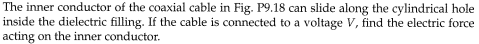
\includegraphics[width=14cm]{p1a}
\end{center}
\end{figure}
\begin{figure}[H]
\begin{center}
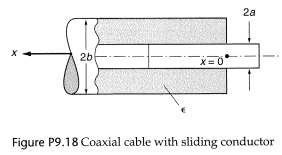
\includegraphics[width=8cm]{p1b}
\end{center}
\end{figure}

The capacitance of a length of cable will be:
\[
  C = \frac{2\pi \epsilon_1 x}{\ln(b/a)} + \frac{2\pi \epsilon_0(L-x)}{\ln(b/a)}
\]

The Electric force will be:
\[
  F = \frac{dW}{dx}
\]
where
\[
  W = \frac{1}{2}CV^2 = \frac{1}{2}(\frac{2\pi \epsilon_1 x}{\ln(b/a)} + \frac{2\pi \epsilon_0(L-x)}{\ln(b/a)})V^2
\]
This means that:
\[
  F = \frac{V^2 \pi (\epsilon_1 - \epsilon_0)}{\ln(b/a)}
\]

\newpage

2) \textbf{10.3:}
\begin{figure}[H]
\begin{center}
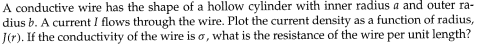
\includegraphics[width=14cm]{p2}
\end{center}
\end{figure}

The current density will be
\[
  J = \frac{I}{A} = \frac{I}{\pi b^2 - \pi a^2}
\]
The resistance of the wire will be $\frac{L}{\sigma A}$ and so the resistance per unit length
will be $\frac{1}{\sigma A}$ or $\frac{1}{\sigma \pi(b^2 - a^2)}$.


\begin{figure}[H]
\begin{center}
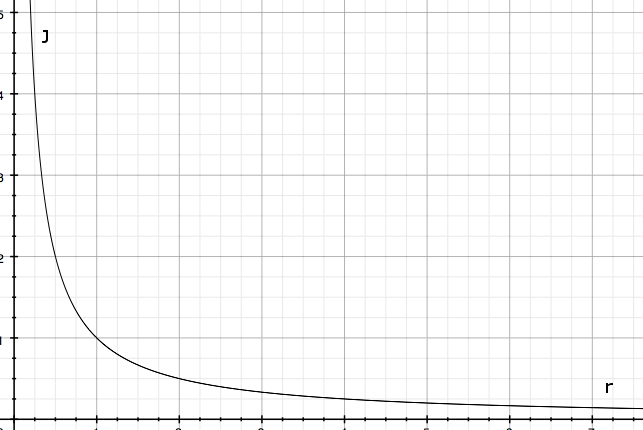
\includegraphics[width=7cm]{graph}
\end{center}
\end{figure}

3) \textbf{10.8:}
\begin{figure}[H]
\begin{center}
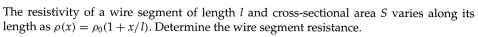
\includegraphics[width=14cm]{p3}
\end{center}
\end{figure}
Since
\[
  \rho(x) = \rho_0(1+x/l)
\]
and
\[
  R = \rho\frac{l}{A}
\]
then
\[
  R(x) = \rho_0(1 + \frac{x}{l})\frac{l}{A}
\]
\[
  R(x) = \frac{\rho_0 l}{A} + \frac{\rho_0 x}{A}
\]

\newpage

4) \textbf{11.11:}
\begin{figure}[H]
\begin{center}
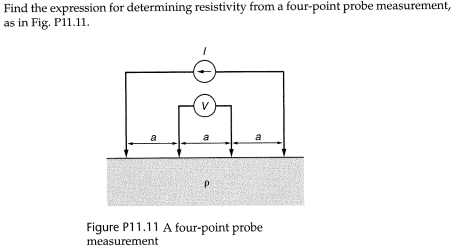
\includegraphics[width=14cm]{p4}
\end{center}
\end{figure}

The potential we are going to measure can be found as in the example problem:
\[
  V_1 - V_2 = \int_a^{2a}[\frac{\rho I}{2\pi r^2} + \frac{\rho I}{2\pi (3a-r)^2}]dr = \frac{\rho I}{2\pi a}
\]
Which becomes:
\[
  \rho = \frac{2\pi a(V_1-V_2)}{I}
\]

\newpage
5) \textbf{12.6:}
\begin{figure}[H]
\begin{center}
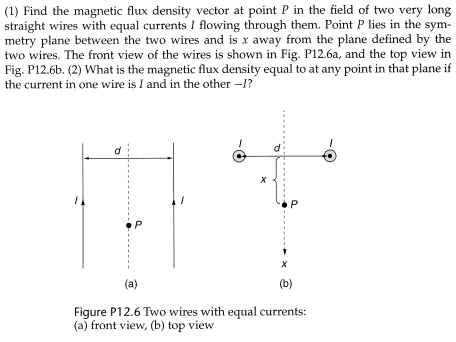
\includegraphics[width=14cm]{p5}
\end{center}
\end{figure}

Using the Biot-Savart law:
\[
  B = \frac{\mu_0}{4\pi}\int \frac{Idl \times u_r}{r^2}
\]
Since there is a field from each wire:
\[
  \frac{\mu_0}{4\pi}\int \frac{Idl \times u_r}{r^2 + (d/2)^2} + \frac{\mu_0}{4\pi}\int \frac{Idl \times u_r}{r^2 + (d/2)^2}
\]
Since the $dl$ components cancel eachother out, and the cross product is 1, we find:
\[
  \frac{\mu_0}{\pi}\frac{Id}{r^2 + (d/2)^2}
\]
in case (b) the magnetic flux density will be the very same, since the vectors from each wire are
the same length, and have the same angle relative to eachother.  The only difference is that it points
int a different direction.

\newpage
6) \textbf{12.7:}
\begin{figure}[H]
\begin{center}
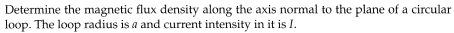
\includegraphics[width=14cm]{p6}
\end{center}
\end{figure}

\[
  B = \frac{\mu_0I}{4\pi}\frac{dl}{r^2}
\]
\[
  B = \frac{\mu_0I}{4\pi}\frac{2\pi a^2}{(z^2 + a^2)^{3/2}} = \frac{\mu_0Ia^2}{2(z^2+a^2)^{3/2}}
\]

7)
\begin{figure}[H]
\begin{center}
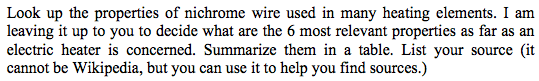
\includegraphics[width=14cm]{p7}
\end{center}
\end{figure}

\begin{center}
\begin{tabular}{| l | l | l |}
  \hline
  Property (name) & Number and unit & Why it is relavant \\
  \hline
  Melting Point & 1475-1710 K & You dont want the heater to get too hot \\
  Resistivity & 84-240$\cdot 10^{-8} \Omega m$ & To find the heater's power useage \\
  Specific Heat & 380-500 J/kgK & To calculate how hot it gets \\
  Thermal Conductivity & 8-17 W/mK & Sounds heater related \\
  Thermal Expansion & 9-16 $10^{-6}/K$ & Also sounds heater related \\
  Elastic Limit & 170-2100 MPa & Important whenever you build something\\
  \hline
\end{tabular}
\end{center}

Everything found here: http://www.nickel-alloys.net/nickel\_chrome\_alloys.html

8)
\begin{figure}[H]
\begin{center}
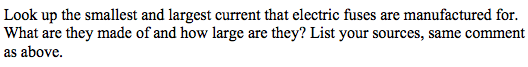
\includegraphics[width=14cm]{p8}
\end{center}
\end{figure}

The largest I could find is 7500A here: http://www.cooperindustries.com/content/
public/en/bussmann/electrical/products/high\_speed\_/square\_body/square\_body\_flushendcontact
size23241000-7500a.html  Its made for power distrobution usage.  The smallest one
I could find is 0.05 Amps, here: http://www.littelfuse.com/products/fuses/axial-radial-
thru-hole-fuses/\~/media/electronics/datasheets/fuses/littelfuse\_fuse\_242\_datasheet.pdf.pdf
Which is for electronics in "explosive" equipment.

\end{document}
